\subsection{Funktionen der App}
        In den folgenden Abschnitten werden jetzt die Funktionen der App dargestellt und erklärt.
        Dazu werden beispielhaft einzelne Methodenimplementationen herausgenommen, erörtert und
        im Kontext der jeweiligen Funktion erklärt.
        Außerdem werden Design-Entscheidungen skizziert um die Nutzer-Erfahrung zu visualisieren.   
    \subsubsection{Rollen und Registrierung}
            Wie bereits in der Zielsetzung angesprochen, soll es ein Berechtigungssystem für die App geben.
            Dieses wird unterteilt in die Rollen Sanitäter/-in und Alarmierende/r. Alarmierende sollen nur in der Lage
            sein einen Alarm auszulösen und die Alarmierenden-News, sowie die Notfallnummern einzusehen.
            Anders als die Alarmierenden sollen Sanitäter/-innen auch in der Lage sein einen Alarm zu empfangen und 
            andere Sanitäter/-innen zu vertreten oder sich aus dem Dienstplan auszutragen.
            Um dies umzusetzen muss bereits bei der Registrierung darauf geachtet werden, wer welche Rolle 
            zugewiesen bekommt.
            Im Folgenden erkläre ich jetzt, zunächst beispielhaft, wie die Registrierung für einen Sanitäter 
            abläuft und erkläre im Anschluss, welche Unterschiede es bei der Registrierung für einen Alarmierenden gibt.
            \newline\\
            Zunächst muss der/die Nutzer/-in den ihr/ihm zugehörigen Sanitätsdienst auswählen.
            Um den Sanitätsdienst auszuwählen muss der / die Nutzer/-in auf den gewünschten Sanitätsdienst wählen. Wenn dieser nicht direkt zu finden ist,
            ist es außerdem möglich diesen mit der Suchleiste oben zu suchen. Im Anschluss muss dann auf den "Weiter"-Button geklickt werden um sich im Anschluss anzumelden oder zu Registrieren.
            Der Button zeigt außerdem an, ob es möglich ist auf diesen zu klicken oder nicht, je nachdem ob bereits ein Sanitätsdienst ausgewählt worden ist oder nicht. Dies wird dadurch angezeigt, 
            dass dieser grau ist, wenn der Button nicht angeklickt werden kann und grün, wenn er angeklickt werden kann.
            \\In Abbildung 1 ist der View zu sehen, in welchem der Sanitätsdienst ausgewählt wird.
            
            %\begin{figure}[H]
            %    \begin{center}
            %       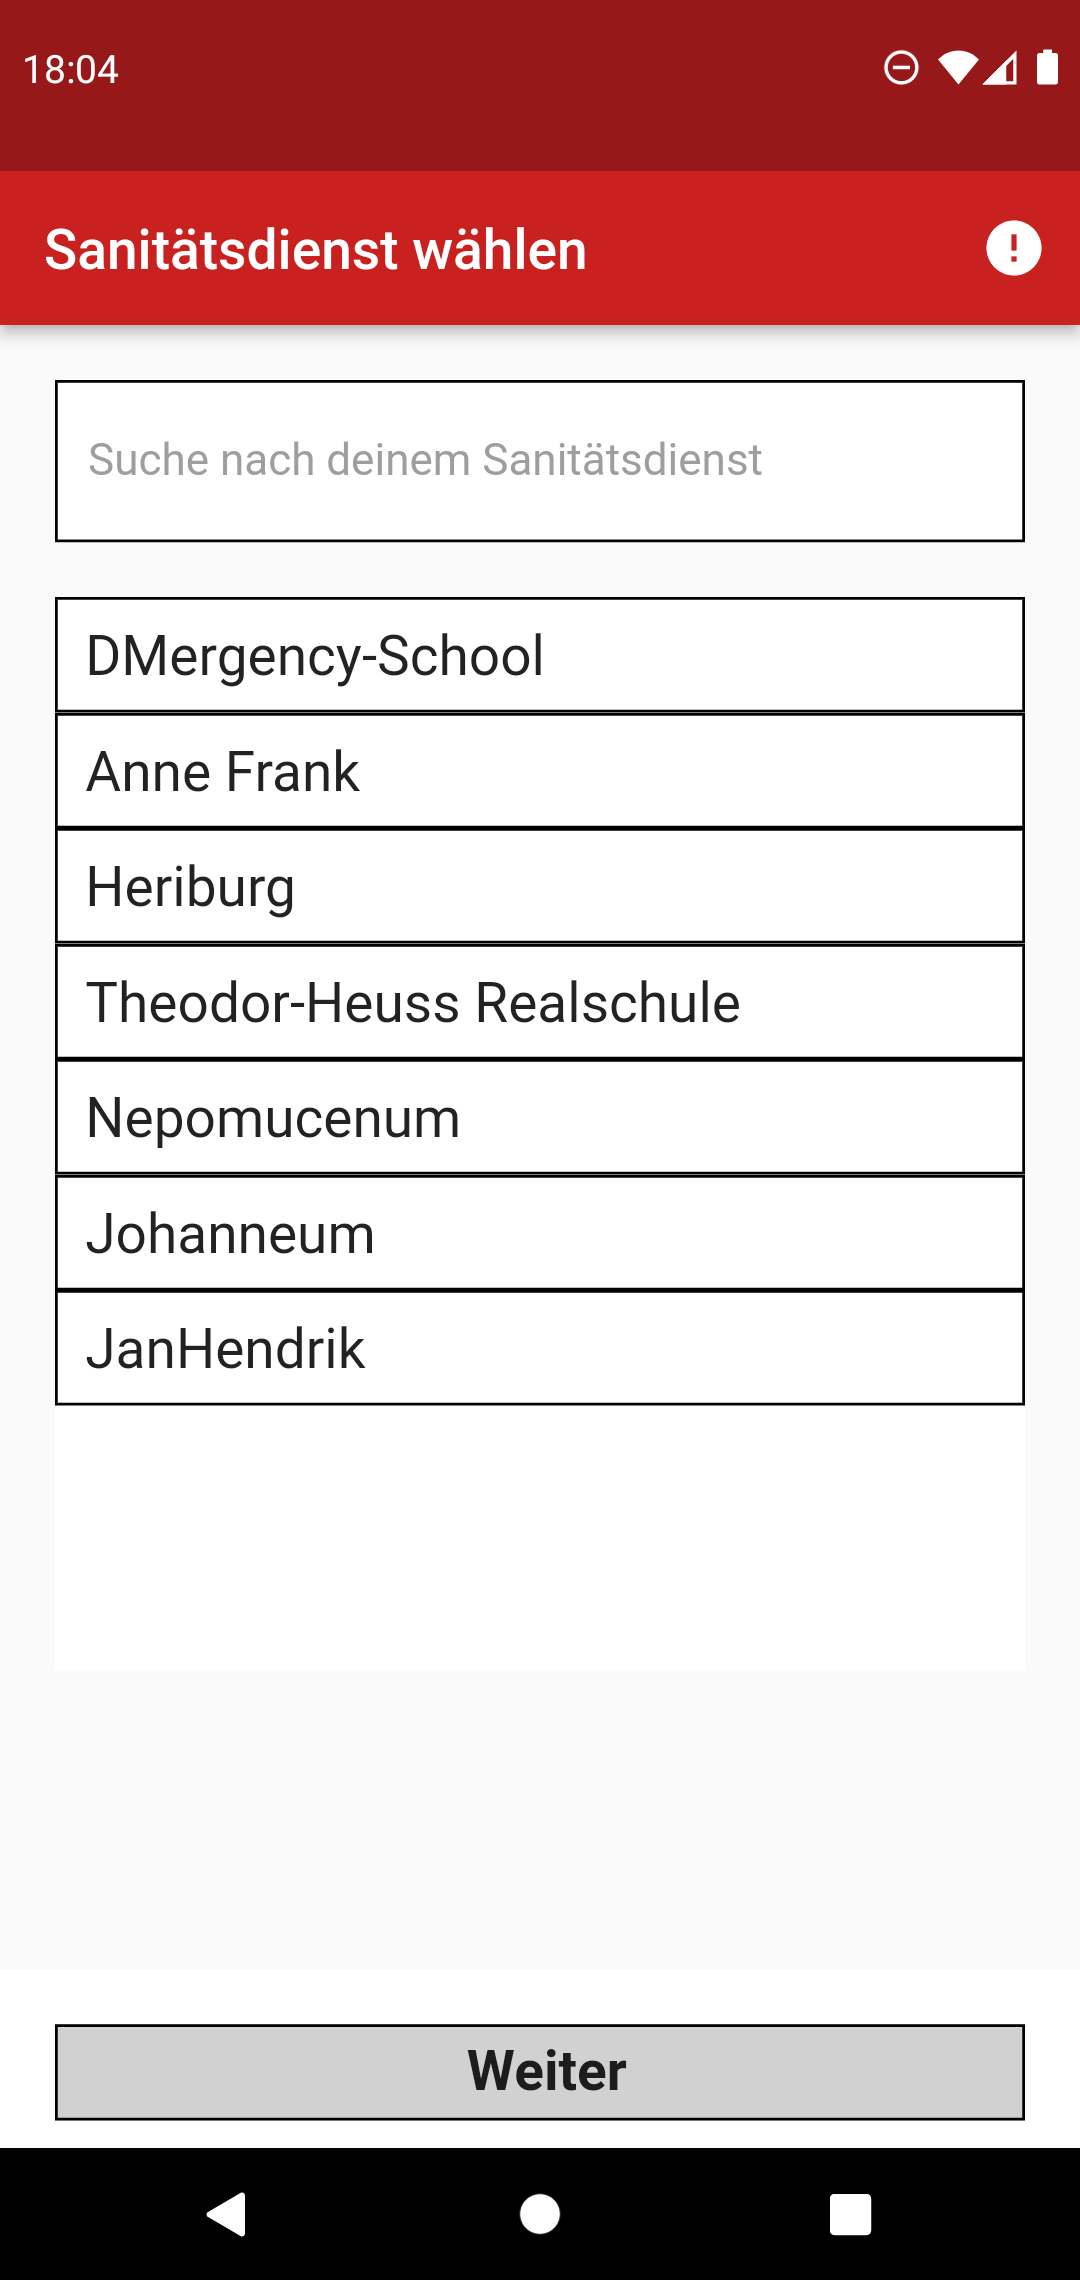
\includegraphics[width = 5cm]{images/SanitaetsdienstWahl.png}
            %    \end{center}
            %    \caption[Screenshot der Sanitätsdienst-Auswahl]{Beispielhafte Sanitätsdienst-Auswahl}
            %\end{figure}
            
            \noindent Um dies umzusetzen muss beim Start der App zunächst überprüft werden 
            ob bereits ein Nutzer eingeloggt ist oder nicht.
            \newline
            1. Es muss überprüft werden ob schon ein Nutzer eingeloggt ist. In diesem \hspace*{5mm}Fall soll keine 
            Sanitätsdienstauswahl angezeigt werden, sondern die nor-\hspace*{5mm}male Nutzeroberfläche, für die entsprechende Rolle.
            \newline
            2. Wenn bisher kein Nutzer eingeloggt ist muss die Sanitätsdienstauswahl \hspace*{5mm}angezeigt werden 
            und die Sanitätsdienste vom Server
            geladen werden.
            \newline\\
            Nachdem der/die Sanitäter/-in dann seinen/ihren Sanitätsdienst ausgewählt hat, soll nun
            ein Login-View angezeigt werden, bei welchem man sich entscheiden kann ob man:
            \newline
            1. sich Einloggen möchte.
            \newline
            2. sich neu Registrieren möchte.
            \newline
            3. sein Passwort vergessen hat und dieses zurücksetzen möchte.
            \newline
            In der Nutzeroberfläche ist dies so umgesetzt, dass je ein Eingabefeld für die E-Mail-Adresse und das Passwort angegeben ist.
            Unter diesem sind dann je zwei Texte, einmal "Registrieren" und einmal "Passwort vergessen", über welche dann auf die unterschiedlichen Views
            geleitet wird.
            Ganz unten in dem View ist dann erneut ein Button, welcher dann zum Anmelden genutzt werden kann. (Auch hier gibt es wieder die Unterscheidung Nutzbar/nicht nutzbar)


            \noindent Um sich anzumelden muss man bereits einen existenten Account besitzen.
            Im Login-View muss man dann seine E-Mail-Adresse, die mit dem Account verknüpft ist, sowie das 
            zugehörige Passwort angeben, um dann eingeloggt zu werden. Die Account-Daten werden nach der Login-Bestätigung
            durch den Nutzer zum Server geschickt und überprüft, um dem/der Nutzer/-in  im Anschluss eine Fehler-Meldung
            anzuzeigen oder sie/ihn auf die Nutzeroberfläche weiterzuleiten.

            \noindent Um sein Passwort zurückzusetzen muss man einen neuen View öffnen, bei welchem man seine E-Mail-Adresse
            angeben kann. Nachdem der/die Nutzer/-in diese bestätigt hat, wird eine E-Mail and die E-Mail-Adresse geschickt, durch die man dann sein Passwort 
            zurücksetzen kann.

            \noindent Das Registrier-Verfahren ist im Gegensatz zum Login und Passwort zurücksetzten komplizierter gestaltet.
            Nach dem Aufruf, dass man einen neuen Account erstellen möchte muss zunächst ein Passwort angegeben werden, dass
            durch den Sanitätsdienst festgelegt wurde. Dieses Passwort unterscheidet sich je nach Rolle die zugeteilt werden soll.
            Das heißt: Nutzer/-in A soll die Rolle Sanitäter/-in bekommen, als gibt er/sie Passwort \glqq xyz\grqq an.
            Nutzer/-in B soll die Rolle Alarmierende/-r bekommen, also gibt die Person Passwort \glqq abc\grqq an.
            \newline
            \noindent Nach der Verifizierung dieses Passworts geht es dann für die beiden Rolle unterschiedlich weiter. 
            \\\\
            \noindent 1. Sanitäter/in
            \newline Zunächst müssen Sanitäter/-innen ihren Vor- und Nachnamen zur Identifizierung für die Sanitätsdienst-Leitung angeben.
            Außerdem muss eine Stufe (bestehend aus drei beliebigen Zeichen) und ein Geschlecht angeben. Diese Daten dienen der Sanitätsdienst-Leitung
            zur Identifizierung und Planung des Sanitätsdiensts.\\
            Danach muss der/die Nutzer/-in eine E-Mail-Adresse und ein Passwort angeben, um sich erneut anmelden zu können und den Nutzer im System eindeutig zu
            identifizieren. Das Passwort muss, um sicherzugehen, dass das Passwort angegeben wurde, was gewünscht ist, zweimal eingegeben werden.
            Im Anschluss daran werden dann App-Berechtigungen abgefragt. 
            In den Betriebssystemen Android und iOS, gibt es zum einen Funktionen, die ohne jegliche weitere Berechtigung genutzt werden können. Jedoch stellen die beiden
            Herausgeber der jeweiligen Betriebssysteme (Google und Apple) auch Funktionen zur Verfügung, welche Berechtigungen benötigen, welche durch den Nutzer der App erlaubt werden müssen.
            Dies dient dem Schutz der Daten der Nutzer der Betriebssysteme.
            Ich habe mich entschlossen einige Berechtigungen abzufragen, damit ich den Nutzern einige Funktionen zur Verfügung stellen zu können.
            Auf Android-Geräten habe ich mich dazu entschlossen die Berechtigung den Nicht-Stören-Modus zu überschreiben abgefragt, damit ich jeder Zeit einen Alarm and die Sanitäter/-innen senden kann
            und auch einen Sound abspielen kann sollte sich das Gerät in einem Stumm-Modus oder dem nicht Stören-Modus befinden.
            Eine weitere Berechtigung auf Android-Geräten ist die Aufhebung der Batterie-Optimierung. Diese soll für die App deaktiviert werden, damit diese dauerhaft im Hintergrund laufen kann und die Alarme
            empfangen kann. Auf iOS-Geräten fordere ich zum einen an, dass ich Mitteilungen senden darf, da dies anders als bei Android eine Berechtigung erfordert, zum anderen
            frage ich die Critical-Alert-Berechtigung ab, damit ich genauso wie bei Android-Geräten den Stumm- und den Nicht-Stören-Modus überschreiben darf.
            %Überprüfen ob ich noch weitere Berechtigungen nutze
            %Warum gibt es die Berechtigungen, warum habe ich mich entschieden diese zuu nutzen
            %\\
            \\\\\noindent 2. Alarmierende
            \\ Alarmierende müssen zunächst ähnlich wie die Sanitäter/-innen einen Accountnamen festlegen. Dieser besteht jedoch nicht aus
            Vor- und Nachname sondern nur aus einem generalisierten Namen, da hier theoretisch auch Accountnamen für feste Räume eingetragen können,
            wie z.B. bei einem Schulsanitätsdienst das Sekretariat. Danach muss genauso, wie bei den Sanitäter/-innen eine E-Mail zur eindeutigen Identifikation eines
            Accounts angegeben werde, über welche auch das Passwort, welches im Anschluss angegeben werden muss, zurückgesetzt werden kann.
            Das Passwort muss genauso wie bei den Sanitäter/-innen zweimal eingegeben werden um die richtige Eingabe von diesem sicherzustellen.
            Im Anschluss muss jetzt nur noch durch das Betätigen des "Registrieren"-Buttons die Registrierung abgeschlossen werden, durch das man dann auf das Nutzer-Interface weitergeleitet wird.


    \subsubsection{Alarmauslösung}
    Das Alarmauslösen, soll wie bereits erwähnt, möglichst einfach für die/den Alarmierende/-n sein, da diese meist Laien sind und sich dadurch in einer
    Alarmsituation so oder so schon in einer Ausnahmesituation befinden und es hier keine große Hürde sein sollte sich Hilfe zu besorgen.

    \noindent Um dies zu bewerkstelligen sind auf dem Server Alarmorte vorgespeichert. Diese werden dann beim Aufruf des Views, auf dem der Alarm gesendet wird heruntergeladen
    und im Anschluss angezeigt.
    Um diese auszuwählen muss der/die Nutzer/-in zunächst einen Ort-Typen aus einem Dropdown-Menü auswählen, welcher dann im Anschluss entscheidet, was als genauer Ort angegeben wird. 
    Die genauen Orte können entweder genau den gleichen Wert haben wie der Ort-Typ, oder eine Auswahl an Objekten, oder eine Zeicheneingabe, welche entweder eine Nummerneingabe
    oder eine Texteingabe sein kann. Diese werden dann entweder als Dropdown-Menü, Eingabefeld oder als nicht abänderbarer Text angezeigt.
    Zunächst muss die Alarmierende Person also den Ort-Typen spezifizieren, danach kann der Nutzer dann den genauen Ort spezifizieren.
    Danach kann der/die Nutzer/-in eine Beschreibung des Geschehens verfassen, damit der/die Sanitäter/-in sich bereits vor dem Eintreffen an der Einsatzstelle
    ein Bild von der Lage machen kann, hierfür wird dann ein Eingabefeld angezeigt, in dem der/die Nutzer/-in die Beschreibung angeben kann. 
    Zuletzt kann der/die Alarmierend/-e eine Priorität zwischen 1 und 5 festlegen um die Dringlichkeit klar zu machen.
    Hierbei ist 1 die niedrigste Priorität und 5 die höchste.
    Diese Prioritäts-Auswahl ist durch RadioButtons dargestellt.

    \noindent Der letzte Schritt, der dann noch ausgeführt werden muss ist die Betätigung des \glqq Alarm senden\grqq-Buttons, welcher dauerhaft sichtbar am unteren Ende des Views angezeigt wird, um problemlos jederzeit alarmieren zu können.

    \noindent Nachdem der Alarm gesendet wurde, was durch den Server geregelt wird, nachdem von der App aus eine Request hierfür gestellt wurde, wird der alarmierenden Person ein 
    View angezeigt, auf welchem Rückverfolgt werden kann, welche/-r Sanitäter/-in den Alarm entweder empfangen, abgelehnt oder bestätigt hat.
    Wenn der Alarm noch nicht empfangen wurde wird, um dies zu symbolisieren ein Ladekreis angezeigt, wenn der Alarm empfangen wurde, wird ein schwarzer Hacken
    angezeigt, wenn der Alarm bestätigt wurde wird ein grüner Hacken angezeigt und wenn der Alarm abgelehnt wurde wird ein rotes Kreuz angezeit.

    \subsubsection{Alarmempfang}
    Um einen Alarm versenden zu können, muss dieser logischerweise auch empfangen werden können. 
    Dies wird über das Cloud-Messaging-System, Firebase Cloud-Messaging, von Google, gelöst.
    Beim Empfangen des Alarms (also der Nachricht von Firebase Cloud-Messaging), wird ein Alarm-Sound abgespielt,
    damit der/die Sanitäter/-in diesen mitbekommt. Im Anschluss werden die Alarm-Daten jetzt in die Datenbank geschrieben.
    Wenn der/die Sanitäter/-in die App nun öffnet, kann diese/-r den View \glqq Alarminfo \grqq öffnen, auf welchem die empfangenen
    Alarme angezeigt werden. Wenn der/die Nutzer/-in jetzt auf den neuesten Alarm klickt werden die Alarminformationen hier erneut, jedoch detaillierter angezeigt.
    Hier kann der/die Sanitäter/-in jetzt auch Rückmeldung auf den Alarm geben, in dem er/sie jetzt den Alarm durch die jeweiligen Buttons ablehnt oder annimmt.
    Die Daten werden in der Reihenfolge Alarmierungszeitpunkt, Ort, Beschreibung, Priorität angezeigt. Dies dient zum einen natürlich der Information des Sanitäters/ der Sanitäterin, 
    zum Anderen soll so auch dem/der Sanitäter/-in gezeigt werden, wann der Alarm gesendet wurde um zu wissen, dass er/sie sich ggf. beeilen muss, da der Alarm, z.B. durch eine schlechte 
    Internet-Verbindung erst verspätet angekommen ist. Nach der Alarmierungszeit ist dann der Ort wichtig, da der/die Sanitäter/-in sich dort möglichst schnell hinbewegen sollte und erst dann sind 
    Beschreibung und Priorität wichtig, da dies nur Zusatzinformationen sind, die der/die Sanitäter/-in so oder so am Einsatzort erheben muss.

    \noindent Die Funktion der Alarm-Rückmeldung ist zum einen zum sicherstellen, der Funktionsfähigkeit der App implementiert worden, 
    zum anderen soll so auch der alarmierenden Person Sicherheit gegeben werden, dass Hilfe kommt um sie in der ihr vorliegenden Ausnahmesituation,
    zu unterstützen / zu helfen.
    Die Alarmrückmeldung erfolgt über die Buttons am unteren Ende des Views. Hier sind zunächst die Buttons "Bestätigen" und "Ablehnen" gegeben, im Anschluss wird dann entweder nur die Rückmeldung, die man selbst
    gegeben hat angezeigt, damit der/die Sanitäter/-in dies überprüfen kann, oder sollte man den Alarm bestätigt haben und noch niemand anderes durch die Betätigung des Buttons "Material holen", gezeigt hat, dass dieser dies übernimmt, 
    wird der Button "Material holen" angezeigt um Beschriebenes anzuzeigen.
    Wenn bereits von jemandem das Material geholt wird, wird dies in einem weiteren Feld angezeigt und anstatt der Buttons wird das Feedback für den Alarm angezeigt.

    \subsubsection{Vertretungen}
    Um die Sanitäter/-innen zu Alarmieren ist auf dem Server ein Dienstplan hinterlegt, welcher bestimmt wer an welchem Tag alarmiert wird. 
    Jedoch kann es auch hier zu Ausnahmesituationen kommen, in denen die eigentlich diensthabende Person nicht in der Lage ist den Dienst zu verrichten.
    Damit hier schnell eine Lösung gefunden werden kann, ist es möglich sich in der App zum einen aus dem Dienst auszutragen, und zum Anderen kann man auch, sollte jemand einem Bescheid gegeben haben, dass
    die Person ihren Dienst nicht verrichten kann, eine andere Person temporär für diesen Tag vertreten.
    Dies wurde so umgesetzt, dass alle diensthabenden Personen in der App, in einer Liste angezeigt werden. Hier kann der Nutzer dann entweder eine der diensthabenden Personen
    vertreten, in dem sie diese auswählt und dann auf Vertreten klickt, oder sich selbst austragen, in dem die Person auf den \glqq Austragen \grqq Button klickt.
    \subsubsection{News \& Notfallnummern}
    Um dem Sanitätsdienst eine gute Kommunikation zu ermöglichen, wurde zusätzlich ein News-Feature implementiert. Hier ist zurzeit nur das anzeigen von den News, die auf 
    dem Server gespeichert sind möglich und nicht das Erstellen von neuen News. Die News werden genutzt um die interne Kommunikation des Sanitätsdienstes zu vereinfachen.

    \noindent Um der alarmierenden Person zusätzliche Sicherheit zugeben ist außerdem ein View implementiert worden, auf dem die wichtigsten Notfallnummern aufgelistet sind,
    damit diese die entsprechende Nummer im Notfall durch anklicken der Nummer anrufen kann und sich nicht unbedingt an diese erinnern muss.
    Es wird hier nach dem Klicken ein AlertView angezeigt, bei dem man dann entscheiden kann ob man tatsächlich die angeklickte Notfallnummer wählen möchte, falls man sich verklickt hat.
    
    \subsubsection{Berechtigungen}
    Um der Sanitätsdienst-Leitung möglichst viel Kontrolle zu geben, was von den Sanitäter/-innen gesehen und getan werden kann gibt es einige Berechtigungen, die auf dem Server gespeichert sind.
    Die einfachste und zugleich schwerwiegendste Berechtigung ist das Sperren von einem Account. Diese Berechtigung ist dafür gedacht, dass, sollte ein/e Sanitäter/-in oder ein/-e Alarmierende/-r die App
    fälschlicherweise Nutzen, oder ähnliches kann dieser gesperrt werden.

    \noindent Es gibt jedoch auch weniger drastische Mittel, mit denen die Nutzer/-innen eingeschränkt werden können, in dem was sie tun.
    Zum einen kann die Berechtigung entzogen werden mit hohen Prioritäten zu alarmieren(z.B. wenn die Person immer mit Priorität 5 alarmiert obwohl dies nicht notwendig wäre),
    oder sollte die Alarmierung so stark ausgenutzt werden, dass die Sanitäter/-innen unnötiger Weise alarmiert werden, kann die Berechtigung entzogen werden zu Alarmieren.

    \noindent Außer bei der Alarmierung gibt es auch Berechtigungen bei dem Vertretungssystem. Hier gibt es die Möglichkeit den Sanitäter/-innen die Berechtigung zu entziehen zu vertreten oder sich aus 
    dem Dienst auszutragen. Ein Anwendungsfall hierfür wäre zum Beispiel das sich ständige Austragen aus dem Dienst aus keinem Grund, oder dem Vertreten anderer Sanitäter/-innen ohne Absprache.

    \noindent Die letzte Möglichkeit Nutzer/-innen einzuschränken ist, die Berechtigung zu entziehen, die eigenen empfangenen Alarme einzusehen.
    Dies könnte zum Beispiel aus dem Grund passieren, dass Alarmdaten an unbefugte Personen weitergegeben wurden und dies nun verhindert werden soll.
    Die Berechtigungen werden beim Server angefragt und dann je nach View umgesetzt. Der JSON-Array, der vom Server geladen wird, kann dann Folgendermaßen aussehen: [101, 102, 201, 202, 301, 302, 303, 304, 707, 708].